\chapter{ Einleitung}


In vielen Bereichen, wie z.B. der Computergrafik oder Simulation, wird zur Modellierung oder der Lösung komplexer Probleme eine  Grundstruktur verwendet, die auf der Vernetzung von Punktmengen in der Ebene beruht. Die erzeugten Netze sind häufig Dreiecksnetze -- sogenannten  Triangulierungen.
Die Triangulierung einer Punktmenge ist dabei nicht eindeutig; je nach Anwendungsfall gibt es bessere und schlechtere Triangulierungen.\\ 
In der Anwendung  sind Delaunay-Triangulierung~\cite{lee:1986:DelaunayTriangulation} aufgrund  ihrer theoretischen Garantien sowie ihrer  vorteilhaften Eigenschaften besonders beliebt. Diese Eigenschaften sind unter anderem die Dualität zum Voronoidiagramm~\cite{aurenhammer:2000:voronoi}, die Vermeidung annähernd kolinearer Dreiecke und die Maximierung  des kleinsten Innenwinkels über alle Dreiecke. Diese Eigenschaften sind wichtig, um in der Weiterverarbeitung Rundungsfehler zu minimieren.\\
Für die Fälle, in denen z. B. der maximale kleinste Innenwinkel einer festen Knotenmenge immer noch zu klein ist, wurden \textit{Delaunay-Refinement-Algortihmen} (siehe Kapitel~\ref{kap:Algorithmus}) entwickelt. Diese Algorithmen verbessern die Qualität einer gegeben Triangulierung  durch inkrementelles Einfügen von Punkten. \\

In die intrinsische Geometrie~\cite{Bobenko:2006:SIGGRAPH,Bobenko:2007:LaplaceBeltrami} wird die Oberfläche eines Objektes ohne Bezug auf das Objekt oder dessen Lage im Raum als abstrakte Flächen beschrieben,  die lokal euklidisch ist und vereinzelt kegelspitzenartige Singularitäten besitzt. Zur Beschreibung dürfen dabei nur Größen verwendet werden, die  innerhalb der Oberfläche gemessen werden können, wie Nachbarschaftsbeziehung, Längen, Winkel u.s.w. Die intrinsische Betrachtung eines Objekts ermöglicht die Anwendung von ursprünglich für die euklidische Ebene entwickelte Verfahren auf die Oberfläche von Objekten. Dies schließt die Delaunay-Triangulierung  \cite{Bobenko:2006:SIGGRAPH} und das Delaunay-Refinement~\cite{Sharp:2019:NIT} ein. \\

Zweidimensionale Triangulierungen sind in  der euklidischen Ebene bereits gut untersucht~\cite{SHEWCHUK:2002:chuws}, lassen sich aber auch zur Repräsentation von dreidimensionalen Objekten verwenden, in dem sie die Oberfläche modellieren (siehe Abbildung \ref{fig:image7}). \\ 

\begin{figure}[H]%{r}{5cm}
    \centering
    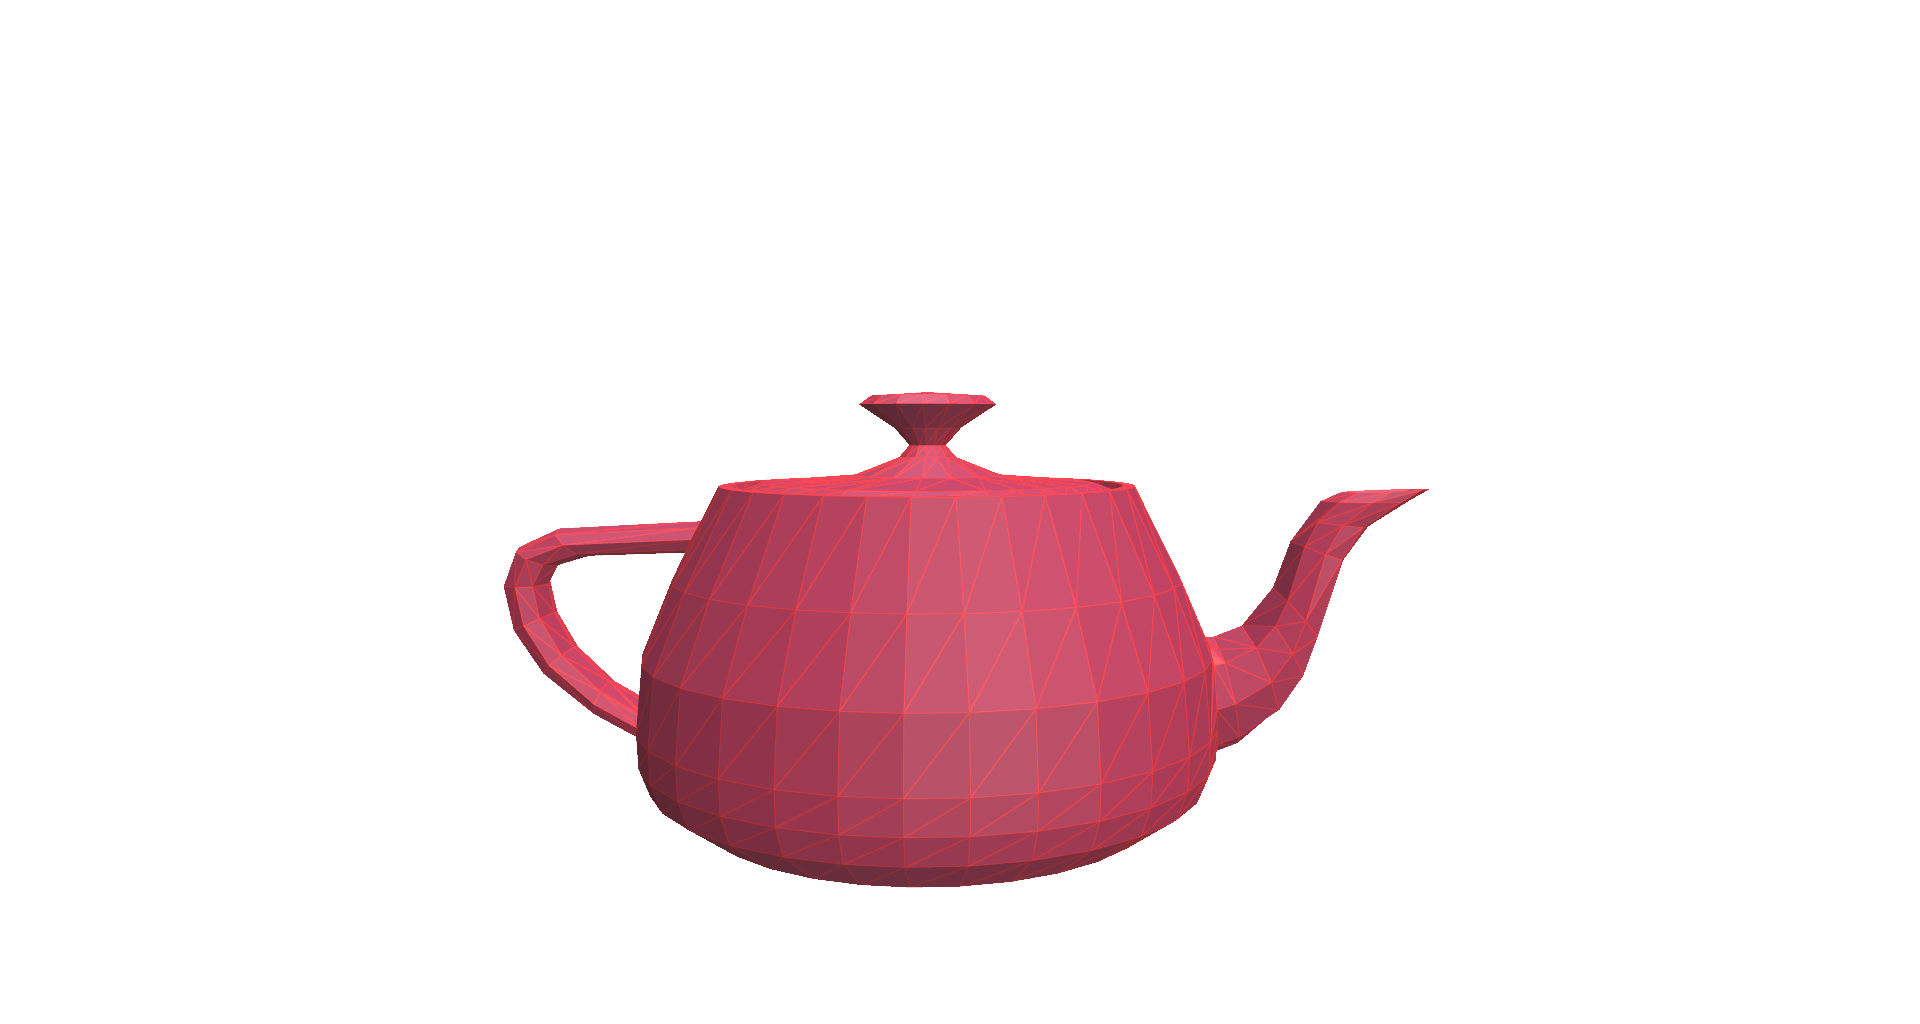
\includegraphics[width=4in]{images/image7.png}
  %\setcapindent{0em}
  \caption{Illustration  der Modellierung von 3D-Objekt durch zweidimensionale Triangulierungen }
  \label{fig:image7}
\end{figure}

Delaunay-Refinement  mit einer Oberflächentriangulierungen als Eingabe hat die Schwierigkeit, dass im Allgemeinen die durch die Optimierung veränderte  Oberflächentriangulierung die geometrische Nähe zum Ursprungsobjekt verliert (siehe Abbildung~\ref{fig:extrinsich_kanten_flip}).\\
\begin{figure}[H]%{r}{5cm}
    \centering
    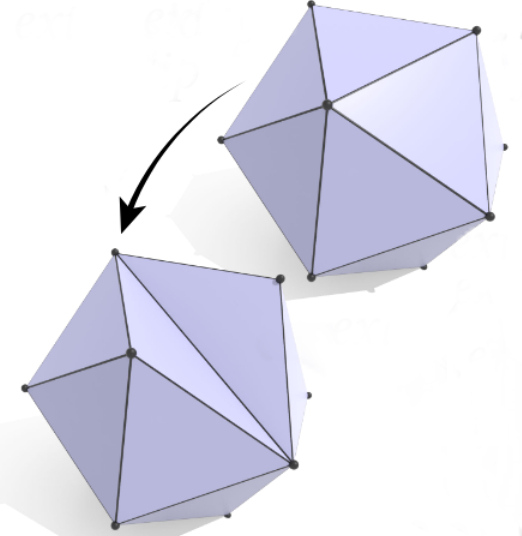
\includegraphics[width=2in]{images/extrinsicher_kantenflip.jpg}
  %\setcapindent{0em}
  \caption{Illustration  dass durch die der Veränderung der Oberflächentriangulierung auch die Geometrie verändert wird~\cite{Sharp:2019:NIT}}
  \label{fig:extrinsich_kanten_flip}
\end{figure}

Beim intrinsischen Delaunay-Refinement  wiederum wird die Eingabe als Triangulierung einer abstrakten Fläche betrachtet, wodurch nur die Triangulierung selbst verändert wird, nicht aber ihre Lage im Raum. Dadurch bleibt die Geometrie des Objekts trotz Veränderung der Triangulierung erhalten.
In~\cite{Sharp:2019:NIT} stellt~\citeauthor{Sharp:2019:NIT} ein Werkzeug für ein intrinsisches Delaunay-Refinement  vor, das sich ausschließlich auf die Qualität der Triangulierung konzentriert, ohne die zugrunde liegende Geometrie zu verändern (siehe Abbildung~\ref{fig:intrinischer_kanten_flip}).\\  


\begin{figure}[H]%{r}{5cm}
    
    \centering
    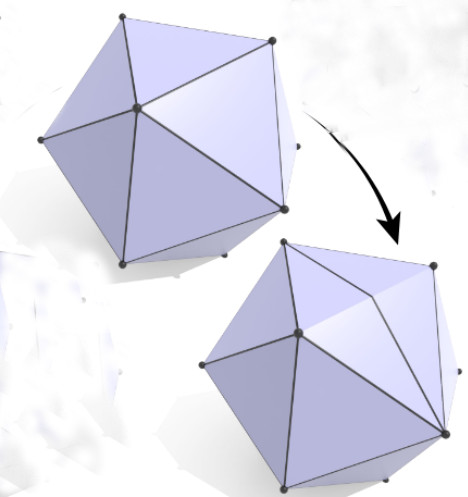
\includegraphics[width=2in]{images/intrinsch_kantenflip.jpg}
  %\setcapindent{0em}
  \caption{Illustration  dass durch intrinsische Veränderung der Oberflächentriangulierung  die Geometrie nicht verändert wird~\cite{Sharp:2019:NIT}}
  \label{fig:intrinischer_kanten_flip}
\end{figure}
\newpage
Das Ziel dieser Bachelorarbeit ist es nun, zu zeigen, welche Einschränkungen bei der Übertragung des Terminierungsbeweises vom planaren Delaunay-Refinement  Verfahren~\cite{chew:1989:guaranteed,ruppert:1995:delaunay,SHEWCHUK:2002:chuws} auf das von  \citeauthor{Sharp:2019:NIT} in   \cite{Sharp:2019:NIT}  vorgestellte intrinsische Delaunay-Refinement  Verfahren auftreten.\\ Dazu werden wir zuerst das traditionelle Delaunay-Refinement  besprechen und vergleichend dazu das intrinsischen Delaunay-Refinement, die Unterschiede zwischen beiden und die daraus resultierenden Schwierigkeiten für den Terminierungsbeweis.\\ 


Der Hauptunterschied liegt hierbei im Winkeldefekt, der bei Oberflächen von Objekten auftreten kann. Ein Winkeldefekt liegt vor, wenn sich die Winkel einer Oberfläche um einen Punkt zu mehr oder weniger als $2\pi$ addieren. Dies kann in der euklidischen Ebene nicht passieren: Hier addieren sich die Winkel um einen Punkt immer genau zu $2\pi$.



Ich zeige in dieser Arbeit, dass ein Winkeldefekt kleiner gleich $\frac{5}{3}\pi$ keine Auswirkungen auf die Terminierung hat. Auf den Umgang mit Segmenten, Größenoptimalität und Aspekte der Abstufung werde ich nur am Rande eingehen.\\










